\documentclass[a4paper,12pt]{article}
\usepackage[slovene]{babel}
\usepackage[utf8]{inputenc}
\usepackage[T1]{fontenc}
\usepackage{lmodern}
\usepackage{amsmath,amsfonts}
\usepackage[ruled,vlined]{algorithm2e}
\usepackage{graphicx}
\usepackage{subfigure}
\usepackage{matlab-prettifier}
\renewcommand{\algorithmcfname}{Algoritem}
\SetKwInput{KwData}{Vhod}
\SetKwInput{KwResult}{Izhod}

\title{\textbf{\huge Simulacija premikanja točke po Bezierjevi krivulji}
	
	\Large \it Poročilo o projektni nalogi pri predmetu Matematično modeliranje}
\author{Nik Erzetič}

\begin{document}
	
	\maketitle
	
	\tableofcontents
	
	\section{Matematično ozadje}
	
	\subsection{B\'{e}zierjeve krivulje}
	
	B\'{e}zierjeve krivulje so parametrične krivulje, določene z zaporedjem kontrolnih točk. Ime nosijo po Pierreu B\'ezierju, ki jih je v drugi polovici dvajsetega stoletja razvil kot orodje za oblikovanje karoserij Renaultjevih avtomobilov.
	
	\subsubsection{De Casteljaujev algoritem}
	
	Osnovno orodje za delo z B\'ezierjevimi krivulji je De Casteljaujev algoritem. Le ta vsaki vrednosti $t$ iz intervala $[0,1]$ (ali $\mathbb{R}$) priredi točko na krivulju. To stori z zaporednim deljenjem stranic in zveznic med v prejšnjem koraku izračunanimi delilnimi točkami, v razmerju določenim s $t$. 
	
	\vspace{3mm}
	\begin{algorithm}[H]
		\KwData{$b_0,b_1,\ldots,b_n \in \mathbb{R}^d$, $t \in [0,1]$ (ali $t \in \mathbb{R}$)}
		\KwResult{točka $b_0^n$ na B\'ezierjevi krivulji}
		definiramo $b_j^0(t) = b_j$, $j=0,1,\ldots,n$
		
		\For{$k=2,3,\ldots,n$}{
			\For{$i=0,1,\ldots,n-k$}{
				$b_i^k=(1-t) \cdot b_i^{k-1} + t \cdot b_{i+1}^{k-1}$
			}
		}
		\caption{De Casteljaujev algoritem}
	\end{algorithm}
	\vspace{3mm}
	
	V Matlabu implementacije ne izgleda tako, a o tem bom več napisal v poznejšem razdelku.
	
	\subsubsection{Odvod B\'{e}zierjeve krivulje}
	
	Odvod B\'ezierjeve krivulje izračunamo po sledeči fomuli:
	$$
	\frac{\mathrm{d}^r b^n}{\mathrm{d}t^r} = n (n-1) \ldots (n - r + 1) \sum_{j=0}^{n-r} \Delta^r b_j B_j^{n-r}(t),
	$$
	kjer je $\Delta b_j = b_{j+1} - b_j$ in $\Delta^r b_j = \Delta (\Delta^{r-1} b_j)$.
	
	\subsection{Fleksijska ukrivljenost}
	
	Fleksijska ukrviljenost $\kappa$ meri upognjenost krivulje v točki. Definirana je kot drugi odvod krajevnega vektorja pri naravni parametrizaciji in je enaka obratni vrednosti radija pritisnjene krožnice v tej točki. Za poljubno parametrizacijo $r(t)$ jo izračunamo z naslednjo formulo:
	
	$$
	\kappa(t) = \frac{\mid r'(t) \times r''(t) \mid}{\mid\mid r'(t) \mid\mid ^3}.
	$$
	
	\section{Reševanje}
	
	Začnimo z De Casteljaujevim algoritmo. V nadaljevanju bom predstavil dva pristopa, a ta algoritem bo ostal enak v obeh primerih.
	
	\begin{lstlisting}[
	style=Matlab-editor,
	numbers=left,
	]
function tocka = deCasteljau(b,t)
  n = size(b,2);
  for i = 2:n
  b = (1-t).*b(:,1:end-1) + t.*b(:,2:end);   
  end
  tocka = b(:,end);
end
	\end{lstlisting}

	Kot vidimo, ga izvajamo na mestu. Vektor $b$ testnih točk rekurzivno manjšamo, dokler nam ne preostane ena sama točka - to je točka na B\'ezierjevi krivulji pri vrednosti $t$.
	
	Prav tako je obema pristopoma skupna sama animacija. V ta namen se uporablja funkcija \lstinline[style=Matlab-editor]!plotBezier!. Le ta izračuna točke v vnaprej določenih vrednostih. Z ukazom \lstinline[style=Matlab-editor]!scatter! nato izrišemo še posamezno točko in njej pripadajočo ukrivljenost.
	
	\begin{lstlisting}[
	style=Matlab-editor,
	numbers=left,
	]
figure;
for i = 1:m
  % Levi zaslon
  subplot(1,2,1);
  hold off;
  plotBezier(b);
  hold on;
  scatter(S(1,i),S(2,i));
  % Desni zaslon
  subplot(1,2,2);
  hold off;
  plot(s,u,'k');
  hold on;
  scatter(s(i),u(i));
  pause(hitrost);
end
	\end{lstlisting}
	
	Ukazi \lstinline[style=Matlab-editor]!figure! in \lstinline[style=Matlab-editor]!subfigure! poskrbijo, da se zaslon loči na dva dela, kjer na levi izrisujemo krivuljo, na desni pa ukrviljenost. V vsaki iteraciji sliko pobrišemo z zlorabo parametrov \lstinline[style=Matlab-editor]!hold on! in \lstinline[style=Matlab-editor]!hold off!.
	
	\subsection{Splošna rešitev}
	
	\subsubsection{Implementacija v Matlabu}
	
	V prvem primeru B\'ezierjevo krivuljo izrišemo tako, da interval $[0,1]$ razdelimo na $m$ delov. V vsaki izmed teh vrednosti potem izračunamo točko po zgoraj zapisanem De Casteljaujevem algoritmu. Na naslednji način izračunamo odvod B\'ezierjeve krivulje:
	
	\begin{lstlisting}[
	style=Matlab-editor,
	numbers=left,
	]
function db = bezier_der(b,r)
  db = b;
  for i = 1:r
  db = (length(db)-1) * diff(db,1,2);
  end
end
	\end{lstlisting}
	
	Tu gre ravno za prej opisano formulo, skrajšano spričo orodji razpoložljivih v Matlabu. 
	
	S pomočjo De Casteljaujevega algoritma nato izračunamo še vrednosti odvoda v vrednostih iz intervala $[0,1]$. Celoten postopek izgleda takole:
	
	\begin{lstlisting}[
	style=Matlab-editor,
	numbers=left,
	]
s = 0:(1/(m-1)):1;
S = [b(:,1) zeros(2,m-2) b(:,end)];
u = zeros(1,m);
db = bezier_der(b,1);
ddb = bezier_der(b,2);
for i = 2:(m-1)
  S(:,i) = deCasteljau(b,s(i));
  dbi = [deCasteljau(db,s(i));0];
  ddbi = [deCasteljau(ddb,s(i));0];
  u(i) = norm(cross(dbi,ddbi),1)/(norm(dbi)^3);
end
	\end{lstlisting}
	
	\subsection{Premikanje z enakomerno hitrostjo}
	
	Če interval $[0,1]$ razdelimo na $m$ enakih delov, se delilne točke ne bodo nujno preslikale v točke na B\'ezierjevi krivulji, ki so med sabo enako oddaljene. Pravzaprav se to, razen v izjemnih primerih, ne bo zgodilo. 
	
	To pomeni, da bo na zgornji način implementirana animacija na delih krivulje pospešila - natančneje na prevojih; izkaže se, da je gostota točk na teh mestih največja.
	
	\begin{figure}[h]
		\subfigure[Poljubna]{
		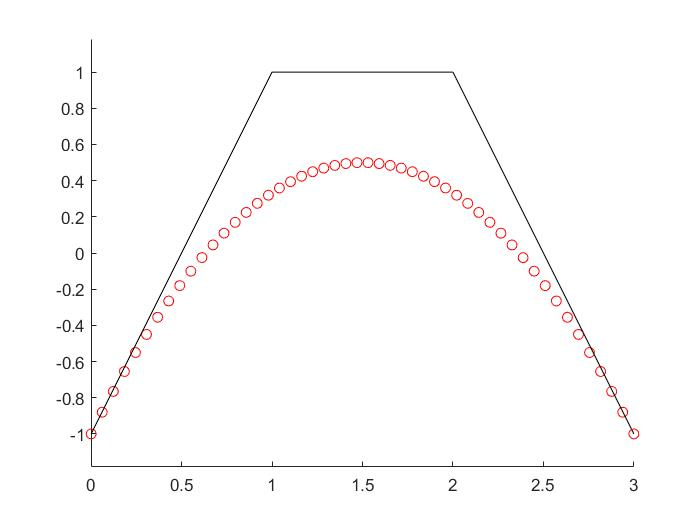
\includegraphics[width=0.5\textwidth]{scatter50normal.jpg}
		}
		\hfil
		\subfigure[Ekvidistančna]{
		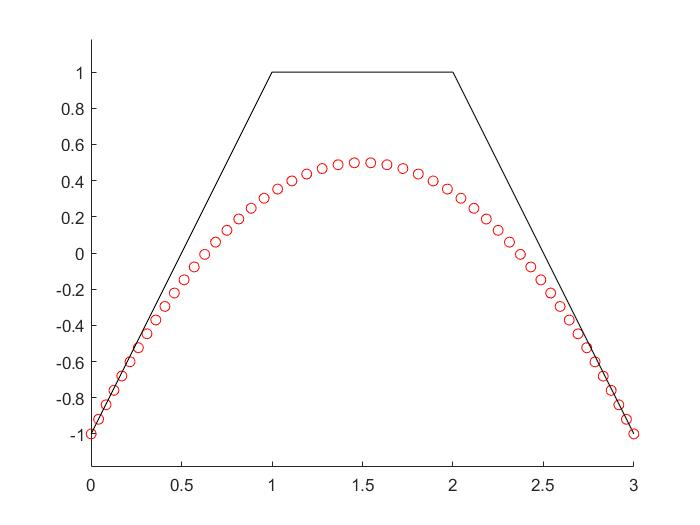
\includegraphics[width=0.5\textwidth]{scatter50eqvi.jpg}
		}
		\caption{B\'ezierjeva krivulja pri poljubni in ekvidistančni parametrizaciji}
	\end{figure}
	
	Le to nam ne najbolj ustreza. Kako hitro se točka premika je izven našega vpliva. Želeli bi, da hitrost lahko nadziramo. Prvi korak do tega pa je enakomerno gibanje. 
	
	\subsubsection{Ekvidistančna parametrizacija}
	
	Na misel nam takoj pade naravna parametrizacija. Vendar je računanje le te nerodno. Prav tako bi to pomenilo, da moramo razširiti interval $[0,1]$ na $[0,L]$, kjer je $L$ dolžina B\'ezierjeve krivulje. To zadnje ne bi bilo preveč zahtevno, a presege namen te projektne naloge. 
	
	Zato se bomo zadovoljili z ekvidistančno parametrizacijo. Pri tej so točke na krivulji nanizane enako daleč ena od druge, kar pomeni, da se bo točka na animaciji premikala z enako veliko hitrostjo.
	
	Tudi ta naloga je vse prej kot enostavna, oziroma zanjo nisem našel nobene elegantne rešitve. Zato sem to dosegel tako, da sem na intervavlu $[0,1]$ minimiziral funkcijo absolutne vrednosti razlike med razdaljo točke od začetka krivulje in željene oddaljenosti:
	
	$$
	f(t) = \mid dolzina(b_0,t) - d_i \mid,\quad i=1,2,\ldots,m-1
	$$
	
	Pri tem sem dolzino med $b_0$ in $t$ aproksimiral s polinomom. Na enak nacin sem izracunal dolžino celotne krivulje $L$ in $d$, ki predstavlja povprečno razdaljo, torej: $d=\frac{L}{m}$. Konstanta na $i$-tem koraku je potem enaka $d_i = i \cdot d$.
	
	\subsubsection{Aproksimacija drugega odvoda}
	
	Druga težava, ki se je pojavila pri takšni parametrizaciji krivulje je, da nimamo direktnega načina za računanje odvodov. To pomeni, da smo odvode primorani aproksimirati. To storimo s kvocientom iz definicije odvoda in izbiro dovolj majnega $h$. Prvi odvod B\'ezierjeve krivulje $b$ je potem:
	
	$$
	b'(t) = \frac{b(t+h)-b(t-h)}{2h}
	$$
	
	Isti trik uporabimo za izračun drugega odvoda, kjer v formulo vstavimo prva odvoda z levo in desno točko:
	
	$$
	b''(t) = \frac{\frac{b(t+h)-b(t)}{h} - \frac{b(t)-b(t-h)}{h}}{h} = \frac{b(t+h)-2b(t)+b(t-h)}{h^2}
	$$
	
	Omenimo še krajišča. V njih nimamo vseh treh potrebnih točk za izračun približka odvodov. Zato privzamemo, da je enaka kot v sosednji točki. Pri zadostnem številu točk napaka ni prevelika.
	
	\subsubsection{Implementacija v Matlabu}
	
	Najprej poiščemo ekvidistančno parametrizacijo. V ta namen definiramo naslednjo funkcijo:
	
	\begin{lstlisting}[
	style=Matlab-editor,
	numbers=left,
	]
function [s,d] = ekvidistancni_parameter(b,m)
  L = dolzinaBezier(b,10*m);
  d = L/(m-1);
  s = zeros(m,1);
  for i = 2:(m-1)
    f = @(t) abs((i-1)*d - dolzinaBezier(b,m,t));
    s(i) = fminbnd(f,0,1);   
  end
  s(m) = 1;
end
	\end{lstlisting}
	
	Funkcija \lstinline[style=Matlab-editor]!fminbnd! poišče lokalni minimum na intervalu $[0,1]$. Dolžino same krivulje aproksimiramo s polinomi. Temu služi funkcija \lstinline[style=Matlab-editor]!dolzinaBezier!
	
	\begin{lstlisting}[
	style=Matlab-editor,
	numbers=left,
	]
function L = dolzinaBezier(b,N,t0)
  t = 0:(t0/(N-1)):t0;
  for i = 2:N-1
    p(:,i) = deCasteljau(b,t(i));
  end
  p = diff(p,1,2); %[dx; dy]
  L = 0;
  for i = 1:N-1
    L = L + norm(p(:,i));
  end
end
	\end{lstlisting}
	
	Ločena funkcija nato iz delilnih točk $s$ izračuna vektor ukrivljenosti. To stori na sledeč način:
	
	\begin{lstlisting}[
	style=Matlab-editor,
	numbers=left,
	]
function u = ukrivljenosti(s,b,d)
  m = length(s);
  u = zeros(m,1);
  h = d/100;
  for i = 2:m-1
    dbi = [(deCasteljau(b,s(i)+h) - deCasteljau(b,s(i)-h))/2/h;0];
    ddbi = [(deCasteljau(b,s(i)+h) - 2*deCasteljau(b,s(i)) + deCasteljau(b,s(i)-h))/h/h;0];
    u(i) = norm(cross(dbi,ddbi),1)/(norm(dbi)^3);
  end
  u(1) = u(2);
  u(m) =  u(m-1);
end
	\end{lstlisting}
	
	Oba vektorja z zgoraj opisanim postopkom izrišemo na vzporednih platnih.
	
	\section{Zaključek}
	
	V projektni nalogi sem implementiral potovanje točke po B\'ezierjevi krivulji. To sem storil na dva načina. Čeprav nam drugi da premikanje z enakomerno hitrostjo, je mnogo počasnejši od prvega. Vsakokratna minimizacija funkcije vzame veliko časa - natančneje vsaj $n \cdot O(n)$. 
	
	Z zmanjšanjem natančnosti bi se morda lahko povečalo hitrost. Prav tako se znotraj različnih funkcij nekateri koraki po nepotrebne ponavljajo. Vendar se, vsaj to drugo, ne da dosti izboljšati.
	
	\section{Viri}
	
	Vsi podatki, navedeni v tem poročilu, izhaja iz mojih zapiskov s predavanj iz Matematičnega modeliranja in Analize 2b na dodiplomskem študiju Matematike, na Fakulteti za matematiko in fiziko Univerze v Ljubljani.
	
\end{document}